% \documentclass[11pt]{aghdpl}
\documentclass[en,11pt]{aghdpl}  % praca w języku angielskim

% Lista wszystkich języków stanowiących języki pozycji bibliograficznych użytych w pracy.
% (Zgodnie z zasadami tworzenia bibliografii każda pozycja powinna zostać utworzona zgodnie z zasadami języka, w którym dana publikacja została napisana.)
% \usepackage[english,polish]{babel}
\usepackage[english]{babel}

% Użyj polskiego łamania wyrazów (zamiast domyślnego angielskiego).
% \usepackage{polski}

\usepackage[utf8]{inputenc}

% dodatkowe pakiety

\usepackage{mathtools}
\usepackage{amsfonts}
\usepackage{amsmath}
\usepackage{amsthm}

% --- < bibliografia > ---

\usepackage[
style=numeric,
sorting=none,
%
% Zastosuj styl wpisu bibliograficznego właściwy językowi publikacji.
language=autobib,
autolang=other,
% Zapisuj datę dostępu do strony WWW w formacie RRRR-MM-DD.
urldate=iso8601,
% Nie dodawaj numerów stron, na których występuje cytowanie.
backref=false,
% Podawaj ISBN.
isbn=true,
% Nie podawaj URL-i, o ile nie jest to konieczne.
url=false,
%
% Ustawienia związane z polskimi normami dla bibliografii.
maxbibnames=3,
% Jeżeli używamy BibTeXa:
backend=bibtex
]{biblatex}

\usepackage{csquotes}
% Ponieważ `csquotes` nie posiada polskiego stylu, można skorzystać z mocno zbliżonego stylu chorwackiego.
% \DeclareQuoteAlias{croatian}{polish}

\addbibresource{bibliography.bib}

% Nie wyświetlaj wybranych pól.
%\AtEveryBibitem{\clearfield{note}}


% ------------------------
% --- < listingi > ---

% Użyj czcionki kroju Courier.
\usepackage{courier}

\usepackage{listings}
\lstloadlanguages{TeX}

\lstset{
	literate={ą}{{\k{a}}}1
           {ć}{{\'c}}1
           {ę}{{\k{e}}}1
           {ó}{{\'o}}1
           {ń}{{\'n}}1
           {ł}{{\l{}}}1
           {ś}{{\'s}}1
           {ź}{{\'z}}1
           {ż}{{\.z}}1
           {Ą}{{\k{A}}}1
           {Ć}{{\'C}}1
           {Ę}{{\k{E}}}1
           {Ó}{{\'O}}1
           {Ń}{{\'N}}1
           {Ł}{{\L{}}}1
           {Ś}{{\'S}}1
           {Ź}{{\'Z}}1
           {Ż}{{\.Z}}1,
	basicstyle=\footnotesize\ttfamily,
}

% ------------------------

\AtBeginDocument{
	\renewcommand{\tablename}{Table}
	\renewcommand{\figurename}{Fig.}
}

% ------------------------
% --- < tabele > ---

\usepackage{array}
\usepackage{tabularx}
\usepackage{multirow}
\usepackage{booktabs}
\usepackage{makecell}
\usepackage[flushleft]{threeparttable}

% defines the X column to use m (\parbox[c]) instead of p (`parbox[t]`)
\newcolumntype{C}[1]{>{\hsize=#1\hsize\centering\arraybackslash}X}


%---------------------------------------------------------------------------

\author{Krzysztof Szczęsny, Jan Twardowski}
\shortauthor{K. Szczęsny, J. Twardowski}

\titlePL{Algorytm do wyznaczania pozycji i orientacji obiektu na podstawie sekwencji wideo.}
\titleEN{Algorithm for visual odometry.}


\shorttitlePL{Algorytm do wyznaczania pozycji i orientacji obiektu na podstawie sekwencji wideo.} % skrócona wersja tytułu jeśli jest bardzo długi
\shorttitleEN{Algorithm for visual odometry.}

%\thesistype{Praca dyplomowa magisterska}
\thesistype{Master of Science Thesis}

%\supervisor{dr inż. Jarosław Bułat}
\supervisor{Jarosław Bułat, PhD}

%\degreeprogramme{Teleinformatyka}
\degreeprogramme{Teleinformatics}

\date{2017}

%\department{Katedra Telekomunikacji}
\department{Department of Telecommunications}

%\faculty{Wydział Informatyki, Elektroniki i Telekomunikacji}
\faculty{Faculty of Computer Science, Electronics and Telecommunications}

\acknowledgements{Serdecznie dziękuję \dots tu ciąg dalszych podziękowań np. dla promotora, żony, sąsiada, żony sąsiada itp.}


\setlength{\cftsecnumwidth}{10mm}

%---------------------------------------------------------------------------
\setcounter{secnumdepth}{4}
\brokenpenalty=10000\relax

\begin{document}

\titlepages

% Ponowne zdefiniowanie stylu `plain`, aby usunąć numer strony z pierwszej strony spisu treści i poszczególnych rozdziałów.
\fancypagestyle{plain}
{
	% Usuń nagłówek i stopkę
	\fancyhf{}
	% Usuń linie.
	\renewcommand{\headrulewidth}{0pt}
	\renewcommand{\footrulewidth}{0pt}
}

\setcounter{tocdepth}{2}
\tableofcontents
\clearpage


\chapter{Theoretical background and state-of-the-art}
\label{cha:intro}


In this chapter theory behind computer vision, 3D reconstruction and mathematical apparatus used in our algorithm are introduced. Pinhole camera model and basics of stereo and mono vision are briefly discussed. Other topics -- Difference of Gaussians edge detection and 3D rotation conventions -- can be found in Appendices B and C, respectively. Literature connected with this topic is overviewed. Finally, \textit{Rebvo} algorithm \cite{jose2015realtime} is described.

%-----------------

\section{Pinhole camera model}
\label{sec:pinhole}

todo: add zhang30 citation

Pinhole camera model is a widely used and simple model that establishes connection between world coordinates $\Re^3$ and image-domain coordinates $\Re^2$ (i.e. projective geometry) \cite{hartley2003multiple}.

\begin{figure}[h]
	\centering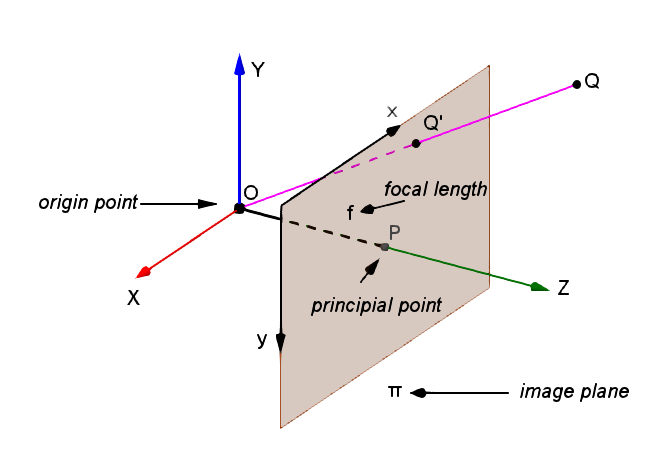
\includegraphics[width=0.6\linewidth]{img/projective.PNG}
	\caption{Image formation in pinhole camera model \cite{szczesny}}
	\label{fig:projective}
\end{figure}

Operation of pinhole camera is depicted in Fig.~\ref{fig:projective}. Every 3D point $Q$ can be associated with a ray $QO$ that passes through camera origin $O$, usually defined as origin of the 3D coordinate system origin. Such ray can be defined with homogeneous coordinates as set of points $\{(X, Y, Z)\}$ that satisfy Eq.~\ref{eq:homo}:


\begin{equation}
(X, Y, Z) = k(Q_x, Q_y, Q_z)
\label{eq:homo}
\end{equation}
where:
\begin{eqwhere}[2cm]
	\item[$k$] real parameter, \(k \neq 0\),
	\item[$Q$] world coordinates point.
\end{eqwhere}

Image plane \(\pi\) is a rectangle parallel to plane \(XOY\). Its distance from origin is equal to \(f\) (focal length). Usually it is assumed that image plane's \(z\) coordinate is positive -- otherwise formed image would be upside down. Point where axis \(OZ\) intersects \(\pi\) is called principal point.

World coordinate points Q are projected onto \(\pi\) as \(Q'\), thus forming a 2D image. This relationship can be concisely written using camera matrix as in Eq.~\ref{eq:camera}.

\begin{equation}
q = Q' \sim \underbrace{ \underbrace{  \begin{bmatrix}
		f_{x} & s & c_{x} \\ 
		0 & f_{y} & c_{y} \\ 
		0 & 0 & 1
	\end{bmatrix}
}_{K} R \left [ I | -t \right ] }_{C} Q
\label{eq:camera}
\end{equation}
where:
\begin{eqwhere}[2cm]
	\item[$q$] 2D point on image plane,
	\item[$Q'$] 2D point on image plane expressed in homogeneous coordinates (3-tuple),
	\item[$Q$] 3D point corresponding to $q$, expressed in homogeneous coordinates (4-tuple),
	\item[$\sim$] equality between homogeneous points,
	\item[$K$] 3x3 intrinsic camera parameters,
	\item[$C$] 3x4 camera matrix,
	\item[$f_{k}$] focal length along axis $k$,
	\item[$s$] skew factor (usually equal to 0),
	\item[$c_{k}$] $k$-coordinate of the principal point,
	\item[$R$] 3x3 rotation matrix between 3D world coordinates and camera coordinates,
	\item[$t$] translation vector between 3D world coordinates and camera coordinates (3-tuple).
\end{eqwhere}

Real cameras do not fully conform to this model \cite{szczesny}. They contain lenses that enlarge field of view (see Fig.~\ref{fig:analogue}). Lens curve passing light rays in a nonlinear fashion (this can be observed in fish-eye cameras \cite{fisheye_endoscopy}). Moreover, lenses themselves are imperfectly made and aligned. Finally, color aberration and CCD sensor quantization noise introduce more nonlinearity \cite{heikkla14}. All these phenomena account for distortions.

\begin{figure}[h]
	\centering\includegraphics[width=0.6\linewidth]{img/camera2.png}
	\caption{Outline of an analogue camera. A digital camera would feature a CCD in place of film. Source: \url{ http://www.mauitroop22.org/merit_badges/images/camera.jpg} }
	\label{fig:analogue}
\end{figure}

Conrady-Brown model \cite{brown8} \cite{Zhang_flexible} is a classical approach to removing geometric distortions. The most significant distortion component is modeled with a radial, even-ordered polynomial, that is centered at the distortion center (usually located in proximity of the principal point). During camera calibration, coefficients of the said polynomial are measured -- they are assumed to be constant\footnote{In fact they can vary with temperature, focus change and over long periods of time \cite{google_calibration}.} for given camera. Then each image taken by the camera can be rectified with inverse distortion field \cite{opencv}. Example of such field is depicted in Fig.~\ref{fig:brown}.

\begin{figure}[h]
	\centering\includegraphics[width=0.6\linewidth]{img/E90vsE9.png}
	\caption{Example of distortion modeled with Conrady-Brown model. Vectors connect distorted pixel positions with their undistorted counterparts and contours mark areas with constant vector length \cite{szczesny} }
	\label{fig:brown}
\end{figure}

% todo @Jan: not sure if this is such a good example: "Mapping resulting from parametric correction in miscalibrated setups"

%---------

\section{Stereo vision}
\label{sec:stereo}

Most implementations of visual odometry systems use two cameras spaced by a constant baseline, that can be determined during stereo calibration. Abundance of such methods can be explained with similarity to how human visual system works \cite{cyganek}. Brain determines depth of seen features by comparing their positions seen by both eyes and taking into account the baseline, i.e. spacing between eyes.

todo image + reference in text

Eq. \ref{eq:fund} describes correspondence between matched points with the fundamental matrix. At least 7 matches are needed to obtain $F$, but usually much more are used so as to mitigate noise \cite{determining_the_epipolar}. When cameras are calibrated, essential matrix $E$ can be calculated with Eq.~\ref{eq:ess}. Essential matrix can be then decomposed into rotation and translation between 3D points registered by both cameras using SVD (1 solution out of 4 has to be chosen). $E$ has scale ambiguity, which can be resolved using baseline in Eq. \ref{eq:disparity} \cite{improving}. It is worth mentioning that baseline can not be determined using autocalibration alone - an object of known dimensions must be measured on images.

\begin{equation}
p_{2}^{T}Fp_{1}=0
\label{eq:fund}
\end{equation}
where:
\begin{eqwhere}[2cm]
	\item[$p_{i}$] point as registered by $i$-th camera, in homogeneous coordinates,
	\item[$F$] 3x3 fundamental matrix.
\end{eqwhere}

\begin{equation}
K_{2}^{T}FK_{1}=E=[t]_{x}R
\label{eq:ess}
\end{equation}
where:
\begin{eqwhere}[2cm]
	\item[$K_{i}$] $i$-th camera intrinsic parameters matrix,
	\item[$E$] 3x3 essential matrix,
	\item[$t$] translation vector $t=[t_{x}\ \ t_{y}\ \ t_{z}]^T$
	\item[$\lbrack t \rbrack _{x}$] skew-symmetric matrix: $\begin{bmatrix}
		0 & -t_{z} & t_{y} \\ 
		t_{z} & 0 & -t_{x} \\ 
		-t_{y} & t_{x} & 0
	\end{bmatrix}$,
	\item[$R$] 3x3 rotation matrix.
\end{eqwhere}

\begin{equation}
Z = \frac{fb}{|p_{1}-p_{2}|}
\label{eq:disparity}
\end{equation}
where:
\begin{eqwhere}[2cm]
	\item[$Z$] world $OZ$ coordinate of the point (i.e. depth),
	\item[$f$] focal length,
	\item[$b$] baseline.
\end{eqwhere}

% -----------

\section{Monocular visual odometry}
\label{sec:mono}

There are three main issues in monocular visual odometry, which will be discussed in this section:
\begin{enumerate}
	\item scale ambiguity,
	\item position drift over time,
	\item egomotion.
\end{enumerate}

In case when only one camera is available, matches between consecutive frames still can be searched for. However, without knowing the 3D transformation, baseline is unknown, so scene can be reconstructed only up to a scale \cite{hartley}. Main difficulty is that this transformation is \textit{the} quantity that odometry is supposed to estimate. Information from only one camera is not sufficient to solve the ambiguity. For instance, Fig.~x depicts a situation when two objects with differing dimensions appear to be of the same size after projection to image plane. There are 2 main ways of alleviating this problem.

todo: figure

An IMU (accelerometer \& gyroscope) -- data from this unit can be used to estimate baseline and extrinsic camera parameters \cite{tracked_vehicles}. Actually, IMU alone can be used for odometry. By combining it with video input, however, accuracy and robustness can tremendously increase.

Another approach is to use explicit depth data, e.g. RGB-D from Kinect \cite{an_improved_visual_odometry_optimization}. This helps in global scene scale estimation. A~disadvantage is that such devices have narrow depth detection range (usually up to few meters \cite{accuracy_and_resoulution}) and are not available in consumer-grade mobile devices.

In \cite{robust_scale} a novel approach is proposed: by assuming a known, constant camera height above ground plane, global scale can be estimated. This step is performed between all consecutive frames, independently from main visual odometry algorithm.

A very frequent problem in pure visual monocular odometry is unbounded position drift over time. Each 3D transformation that is estimated between consecutive frames is an instantaneous linear and angular velocity. To obtain accumulated position and azimuth after given frame, individual velocities have to be integrated. Each estimation error gains significance with time. In literature two ways of mitigation are the most common.

% todo: demonstration of this conjecture?

First of all, information from GPS can be employed to ensure that position does not drift away \cite{accurate_global_localization}. GPS signal quality greatly depends on location, so this approach may be unsuited for indoor use cases. GPS can not help with azimuth estimation, however. Finally, GPS is, out of the discussed methods, the only way to transform relative coordinates to real word coordinates (i.e. longitude and latitude). Other possibility would be to use special markers.

In SLAM systems loops in trajectories can be used as means of correcting position drift -- knowing landmark\footnote{Landmark is an excellent feature point, observable from many frames.}) descriptors in past frames, such loops can be detected and system parameters can be adjusted to close them \cite{the_application_of_kalman} \cite{monoslam}.


todo: egomotion \& "tunnel" motion
\cite{vehicle_egomotion} \cite{recovery_of_egomotion}


%---------


\section{Literature}

todo:

\cite{visual_odometry} - landmark paper

\cite{fast_monocular} - outlier removal

\cite{spatiotemporal} - good for full SLAM

\cite{a_kalman}

\cite{monoslam} - SLAM using only camera, new approach (camera is not on a robot, but independent)

\cite{real_timeLocalization}

\cite{robust_visual_odometry_estimation} - dense method

\cite{semi_dense} - semi-dense method

\cite{a_stereo_visual} - comparison of feature detectors, consistency check

% -------------

\section{The \textit{Rebvo} algorithm outline}

In this section the \textit{Rebvo} algorithm \cite{jose2015realtime} description is briefly paraphrased for needs of this thesis.

\textit{Rebvo} is a novel approach to monocular visual odometry. The algorithm is capable of running in real time on an ARM processor \cite{jose2015realtime}. It is similar to semi-dense methods, that achieve SLAM using only selected features (in this case -- edges). It is not a full SLAM system, so only two consecutive frames are stored at each time and no global map is created. Information from previous frames is retained as estimated depth. Features are matched on pixel basis. This concept is compliant with argument made in \cite{harris}: TODO quote or paraphrase.

Algorithm consists of three main steps, similar to other visual odometry systems. First of all, \textbf{edge extraction} is performed, preferably with subpixel precision. Moreover, edge gradient is calculated for each pixel. Neighboring pixels are joined into connected\footnote{Each edge has no gaps between neighboring pixels} edges, using gradient information.

Then \textbf{tracking} is performed. Edges from previous frames are first projected into 3D space using their already estimated depths. Then an iterative procedure (Levenberg-Marquardt algorithm) aims to find such 3D transformation that establishes consensus between frames. Projected points are rotated and transformed in 3D, then projected back onto image plane. Minimized cost function is essentially the sum of squared distances between back-projected edges from the previous frame and closest edges from the current frame. Actual cost function also takes into consideration gradient correspondence criteria. Obtained pairs of edge pixels do not constitute an exhaustive list of matches, because:
\begin{itemize}
\item transformation is not ideal,
\item depth of pixels is only estimated,
\item there is quantization noise,
\item edges can be detected inconsistently between frames (todo cite),
\item even for undistorted images, some residual distortion noncompliant with pinhole camera model will be present \cite{barreto2007non},
\item outliers can be present (e.g. objects moving with respect to the otherwise rigid scene).
\end{itemize}
 
Final step -- \textbf{mapping} -- associates matching edges between frames using obtained optimal 3D transformation. Due to aforementioned problems, after tracking a matching routine is needed for each edge pixel. Because depth of previous frame edges is estimated with some uncertainty, camera motion establishes a line segment defining the area where possible matches will be searched for. Once a candidate has been found, it is tested for gradient correspondence and, most importantly, for model consistency~\==~deviation of position on the segment obtained from linear transformation equation can not exceed depth uncertainty. After matching, depth information is propagated for matched edge pixels from previous frame to the current, and is optionally regularized. Previous depth has to be reestimated ($OZ$ axis velocity has to be taken into account). This is achieved using Extended Kalman Filter. Scale drift, inherent problem of pure visual odometry, can be then mitigated to some limited degree by diving estimated depths by frame shrinking factor.

Accuracy of results obtained in \cite{jose2015realtime} are comparable with other state-of-the-art algorithms. todo: cite \cite{yang2017direct}

% ---


\chapter{Analysis and improvements of \textit{Rebvo} algorithm}
\label{cha:intro2}

This chapter contains thorough analysis of proposed algorithm. The algorithm is carefully explained, step by step, using various examples. Symbols used through the chapter are explained in Section~\ref{sec:struct}. Much attention is paid to edge detector, because it also had to be implemented, as available ready-made edge detection methods did not meet algorithm requirements. Figures used throughout the chapter were generated using input images from TUM \cite{tum} and KITTI~\cite{kitti} datasets. Chapter is concluded with remark on trajectory postprocessing, used to estimate algorithm accuracy.

Note: considerations, improvements and modifications of the original algorithm are \textbf{emphasized}.

\section{Notation (Keyline structure) and {\tt main} loop}
\label{sec:struct}

Pixels that contain subpixel edge positions are called Keylines and, after edge extraction, are stored as an array of structures defined in Table \ref{tab:keyline}. When $(n+1)$-th frame of video input is being processed, only $n$-th and $(n+1)$-th Keyline arrays are available; $(n-1)$-th is discarded, as it is no longer needed. This is presented in Fig.~\ref{fig:flowchart_main}. Fields of $n$-th Keyline array will be denoted with subscript $_{p}$ (for \textit{previous}) and $_{t}$ (for \textit{transformed}). Subscripts $_{c}$ (\textit{current}) and $_{r}$ (\textit{rotated}) will be associated with $(n+1)$-th frame.

\begin{figure}[hp]
	\begin{footnotesize}

	\centering\begin{tikzpicture}[node distance = 2cm, auto]
	% Place nodes
	
	\node [cloud] (start) {start};
	\node [block, below of=start] (b0) {{\tt n := 1}};
	\node [block, below of=b0] (b05) {{\tt parameters\_initialization()}};
	\node [block, below of=b05] (b1) {{\tt KLs\textsubscript{p} := edge\_detection(n) }};
	
	\node [block, below of=b1] (b2) {{\tt n++}};
	\node [block, below of=b2] (b3) {{\tt KLs\textsubscript{c} := edge\_detection(n) }};
	
	\node [block, below of=b3] (b4) {{\tt edge\_tracking()}};
	
	\node [decision, below of=b4] (b5) {minimization successful?};
	
	\node [block, below of=b5, node distance=8.5em] (b6) {{\tt mapping()}};
	
	\node [decision, below of=b6, node distance=8.5em] (b7) {\\*$card(KLs_{new}.m_d) > 500$?};
	
	\node [block, right of=b5, text width=10em, xshift=10em] (b8) {{\tt KLs\textsubscript{p} := KLs\textsubscript{c}}};
	% Draw edges
	
	\path [line] (start) -- (b0);
	\path [line] (b0) -- (b05);
	\path [line] (b05) -- (b1);
	\path [line] (b1) -- (b2);
	\path [line] (b2) -- (b3);
	\path [line] (b3) -- (b4);
	\path [line] (b4) -- (b5);
	\path [line] (b5.west) -| node [near start] {no} ([xshift=-1cm] b05.west)
	                       |- (b05.west);
	\path [line] (b5.south) -- node {yes} (b6);
	\path [line] (b6) -- (b7);
	\path [line] (b7.west) -| node [near start] {no} ([xshift=-1cm] b05.west)
					   	   |- (b05.west);
	\path [line] (b7.east) -| node [near start] {yes} (b8.south);
	\path [line] (b8.north) |- (b2.east);
	\end{tikzpicture}
	
	\caption{Simplified flowchart of the algorithm. $KLs_{x}$ are arrays of Keyline structures}
	\label{fig:flowchart_main}
		\end{footnotesize}
\end{figure}

\begin{table}[ht]
	\centering
	
	\begin{threeparttable}
		\caption{Keyline structure}
		\label{tab:keyline}
		
		\begin{tabularx}{1.0\textwidth}{C{0.25} C{0.75}}
			\toprule
			\thead{Structure field} & \thead{Description} \\
			\midrule
			$q = [q_{x},\ q_{y}]^T$ & subpixel position in image \\
			$h = [h_{x},\ h_{y}]^T$ & normalized\tnote{a} $q$: $h = q - [c_{x},\ c_{y}]^T$ \\
			$\rho$, $\sigma_{\rho}$ & estimated inverse depth: $\frac{1}{Z}$, and its variance \\
			$\rho_0$, $\sigma_{\rho_{0}}$ & inverse depth predicted by Kalman filter and its variance \\
			$\vec{g}$ & edge gradient obtained from DoG \\
			$p_{id}, n_{id}$ & index of previous and next Keyline in an edge \\
			$m_f$ & index of next frame Keyline obtained during forward matching \\
			$m_d$ & index of next frame Keyline obtained during directed matching \\
			$k$ & number of consecutive frames that this Keyline has appeared on \\
			\bottomrule
		\end{tabularx}
		
		\begin{tablenotes}
			\footnotesize
			\item[a] Usage of normalized coordinates is more robust \cite{hartley1997defense}. In the implementation, $h$ is also often temporarily divided by $f$, so that calculations on homogeneous coordinates are more stable.
		\end{tablenotes}
		
	\end{threeparttable}
\end{table}

% ---

\section{Edge extraction}

Primal step of algorithm is subpixel edge extraction. Keyline structures are populated using extracted data (edge position and edge gradient). Keylines that are estimated to lie on same edge are joined.

\subsection{Edge detection algorithm choice}
While many edge detection algorithms could be used in this step, authors of \textit{Rebvo} have chosen DoG (Difference of Gaussians), because it provides \cite{jose2015realtime}:
\begin{enumerate}
	\item repetivity -- an edge is detected similarly throughout consecutive frames,
	\item precision -- edge positions are accurate,
	\item low time \& memory complexity.
\end{enumerate}

Another advantage of DoG, unmentioned by Tarrio and Pedre, is that \textbf{edge gradient can be obtained directly} from normal vector of the fitted local plane. In this thesis DoG was used as well. Most vital property was subpixel precision, otherwise Canny detector \cite{canny} would be employed. In principle, subpixel edge detection precision is possible, because as long as Whittaker–Nyquist–Kotelnikov–Shannon theorem assumptions are satisfied, the true continuous image intensity function can be reconstructed from discrete pixel values.

\subsection{Data preprocessing}

First of all, RGB images are converted to grayscale. Color information is not used in the algorithm.

Before performing any edge detection technique, one critical issue has to be addressed. If input images were rectified\footnote{If images were \textit{not} rectified, they should be.} in such a way that extrapolation beyond original borders had been needed, artificial edges will be present in every frame (because extrapolation procedure usually assumes 0 pixel intensity beyond the image). Gradient of these edges is almost always strong, meaning that they tend to pass all tests and to be identified as valid keylines, thus generating false positives. During later minimization step, they greatly distort the procedure, making it behave as if the 3D space was curved. Example of such border is depicted in Fig.~\ref{fig:rectifcy_border}.

\begin{figure}[ht]
	\centering\includegraphics[width=0.75\linewidth, trim={1cm 1cm 1cm 1cm},clip]{img/figures/rectified_edge.png}
	\caption{ Input image, zoomed-in near left border. Individual pixels produced by rectification can be observed on the right }
	\label{fig:rectifcy_border}
\end{figure}

In case of DoG, these \textbf{artificial edges need to be removed} before Gaussian blurring~\==~otherwise they would spread out, making it tricky to reject them later. In tested datasets, artificial borders' thickness did not exceed 1~pixel, so simply 1-pixel wide frame of outermost pixels was always discarded. In general case, \textbf{width of the frame can be figured out from distortion model}, instead of being set manually. However, for highly distorted images, a rectangular frame would also discard many valid pixels -- either in corners (barrel distortions), or near middle of borders (pincushion distortions).

\subsection{Difference of Gaussians strength tests}

After necessary preprocessing, edge detection can be started. Generally edge detection works by finding positions in image where pixel intensity changes most rapidly. Basic idea of DoG is to approximate image second derivative (the Laplacian) \cite{szeliski} \cite{jain1995machine}. The zero-crossing of Laplacian corresponds to such positions. Example based on real data, reduced to one dimension for clarity, is presented on Fig.~\ref{fig:slice}. Other approaches to edge detection involve curve fitting \cite{fabijanska} \cite{devernay1995non} \cite{wei2010two}.

\begin{figure}[ht]
	\centering\includegraphics[width=0.75\linewidth, trim={1.5cm 1.5cm 1.5cm 1.0cm},clip]{img/figures/subpixelslice.png}
	\caption{ DoG zero-crossing subpixel edge detection. Discussed method was applied to an image, then one row of pixels containing very apparent edge was extracted. Red $\times$ denotes calculated subpixel edge position }
	\label{fig:slice}
\end{figure}

In order to filter out noise, image should be first smoothed with a Gaussian filter. These operations can be combined into one operator -- Laplacian of Gaussian -- which in turn can be approximated with difference of two images smoothed with Gaussian filters using two different sigmas\footnote{LoG is best approximated by DoG when $\frac{\sigma_{1}}{\sigma_{2}} = \sqrt{2}$ \cite{sift}.} Edge detection results for initial sigma values were satisfactory in performed tests, therefore other sigma values (or automated sigma adjustment schemes) were not tested.

Exemplary Difference of Gaussians image is depicted in Fig.~\ref{fig:dog}. \textit{Implementation insight}:~while individual smoothed images can be computed using {\tt uint8} as underlying data type (for speed), the difference has to be computed using signed data type. Otherwise obtained function will not cross zero!

\begin{figure}[ht]
	\centering\includegraphics[width=0.75\linewidth, trim={1.25cm 1.25cm 1.25cm 1cm},clip]{img/figures/dog.png}
	\caption{ Difference of Gaussians applied to an image from the TUM dataset~\cite{tum}. Near-zero values indicate feasible edge candidates }
	\label{fig:dog}
\end{figure}

Another parameter is window size -- it defines pixel neighborhood that will take part in later calculations of edge position. For window size $w$, $(2w+1)^2$ immediate neighbors will be considered, including the center pixel itself. For sake of this thesis, value $w = 2$ was used.

\subsubsection{First test}
\label{edge_first}

Edge detection procedure is performed for every pixel that lies at least $w$ pixels from image border, so that neighborhood does not need to be extrapolated. In order to speed up computations by early identifying non-edges, first derivative of pixel intensity is calculated by applying two Sobel operators (derivatives along $x$ and $y$ axes) and taking norm of the result. This norm is then compared with a threshold. 

Tarrio and Pedre use hysteresis to determine threshold value after every frame. On the one hand, presented algorithm operates offline, so abundance of keylines is not an issue. On the other, hysteresis parameters still need to be adjusted for given dataset. Invalid parameters can alter overall algorithm results significantly, so from algorithm analysis point of view, the fewer of them, the better. \textbf{Thus instead simpler solution was tested out}.

Image is partitioned into $a^2$ rectangular chunks, for relatively small $a$, e.g. 7. Then for each chunk number of pixels that would pass the first derivative test for given constant threshold is counted. If this number is relatively low, threshold is locally multiplied by a constant ${b_{1} < 1}$, e.g.~$\frac{1}{3}$. However, if the number is relatively large, then threshold is locally multiplied by ${b_{2} > 1}$,~e.g.~$\frac{5}{3}$. Local threshold array can finally be smoothed with Gaussian filter to avoid discontinuities.

Proposed procedure also has parameters, but there are few advantages:
\begin{itemize}
	\item parameters are much simpler to interpret,
	\item effectively only one parameter is crucial (the constant threshold) and rest of procedure serves as a refinement,
	\item operates without delay, which is vital especially if keyline number is too low.
\end{itemize}

In Fig.~\ref{fig:bucket} some pixels on the right half of the image were considered further for being edges, although ultimately they were also rejected. On the other hand, more non-edge pixels have been rejected by the first test on the left half (green regions are a bit thinner). However, if any edges \textit{are} added by this method, they are not very stable and tend to be nonetheless untraceable in later frames (they do not exhibit the \textit{repetivity} property).

\begin{figure}[ht]
	\centering
	\begin{subfigure}{1\textwidth}
		\centering
		\centering\includegraphics[width=0.8\linewidth]{img/figures/02_0013.png}
		\subcaption{\label{fig:bucket_a}}
	\end{subfigure}
	\begin{subfigure}{1\textwidth}
		\centering
		\centering\includegraphics[width=0.8\linewidth]{img/figures/02_0013_bucket.png}
		\subcaption{\label{fig:bucket_b}}
	\end{subfigure}
	\caption{\label{fig:bucket} Edge detection tests results. Pixel colors: dark blue -- neighborhood outside image; blue, light blue (not present), cyan (not present), green and orange -- rejected by tests 1 to 5, respectively; red -- reserved for debug purposes (not present); dark red -- final Keylines. \protect\subref{fig:bucket_a} Constant first test threshold,
		\protect\subref{fig:bucket_b} Chunked first test threshold}
\end{figure}

\subsubsection{Second test}
\label{edge_second}

Neighborhood of pixels that have passed the first test is checked for ``sign balance``. Number of positive and negative DoG values has to be comparable within a defined percentage, e.g. 20\%. Example results of the test for 2 different pixels are depicted in Fig.~\ref{fig:plusminus}. It was observed that pixels very rarely fail this particular test.

\begin{figure}[ht]
	\centering\includegraphics[width=0.75\linewidth, trim={1.5cm 2.5cm 1.5cm 2.5cm},clip]{img/plusminus.png}
	\caption{ Example of the DoG sign balance test. Negative values are denoted as black pixels, postive -- as white. Green color marks neighborhood of pixel that has passed the test and is, possibly, an edge. Pixel marked with red was rejected }
	\label{fig:plusminus}
\end{figure}

\subsubsection{Third test}
\label{edge_third}

Then DoG values are approximated by a plane using linear regression -- (\ref{eq:regress}) is solved for~$\theta$. Pseudo-inverse of $\tmmathbf{A}$, needed to solve it, has to be computed only once for the whole algorithm. Zero-crossing of the plane can be determined algebraically, resulting in (\ref{eq:zerocross}). This has been visualized in Fig.~\ref{fig:zeroc}. These closed-form formulas are the main reason for DoG not being computationally demanding, as curve-fitting approaches are usually iterative.

\begin{figure}[ht]
	\centering\includegraphics[width=0.75\linewidth, trim={1.0cm 0.5cm 1.0cm 0.5cm},clip]{img/figures/zeroc.png}
	\caption{ Zero-crossing search. DoG values have been depicted with a mesh. Two planes are present: approximation of the DoG and the $z=0$ plane }
	\label{fig:zeroc}
\end{figure}

For more resilience, an additional test is performed. If (\ref{eq:test3}) is not satisfied, then equation system~\ref{eq:regress} \textbf{is considered to be badly conditioned} and this pixel is rejected. This was not considered in \cite{jose2015realtime}. The purpose of this test is to avoid divide-by-zero errors in fourth test (Section~\ref{edge_fourth}). All pixels that do not pass the third test would still be filtered out later -- they also do not pass the fifth test~(Section~\ref{edge_fith}).

\begin{equation}
\tmmathbf{A}\theta = \delta
\label{eq:regress}
\end{equation}
where:
\begin{eqwhere}[2cm]
	\item[$\tmmathbf{A}$] 3x$(2w+1)$ matrix of pixel positions: $[X\ Y\ 1]$,
	\item[$X$] column vector of $x$ coordinates of pixel centroids in neighborhood, assuming that central pixel's centroid is located at $x = 0$, ($(2w+1)$-vector),
	\item[$Y$] column vector of $y$ coordinates of pixel centroids in neighborhood, assuming that central pixel's centroid is located at $y = 0$, ($(2w+1)$-vector),
	\item[$\delta$] DoG values corresponding to $X$ and $Y$ ($(2w+1)$-vector),
	\item[$\theta$] parameters defining the approximated plane: $z = \theta_{x}x + \theta_{y}y + \theta_{z}$.
\end{eqwhere}



\begin{equation}
\begin{bmatrix}
x_s \\
y_s 
\end{bmatrix} = 
\begin{bmatrix}
\frac{-\theta_{x} \theta{y}}{\theta_x^2 + \theta_y^2} \\
\frac{-\theta_{y} \theta{y}}{\theta_x^2 + \theta_y^2}
\end{bmatrix}
\label{eq:zerocross}
\end{equation}
where:
\begin{eqwhere}[2cm]
	\item[$k_s$] estimated $k$-coordinate of the subpixel edge position (0 is the pixel center).
\end{eqwhere}

\begin{equation}
\theta_{x}^2 + \theta_{y}^2 > 10^{-6}
\label{eq:test3}
\end{equation}

\subsubsection{Fourth test}
\label{edge_fourth}

Obtained zero-crossing marks the subpixel position of the edge; an example of a few subpixel positions along an edge is presented in Fig.~\ref{fig:quiv}. (\ref{eq:subpix_inside}) tests whether it lies within the pixel itself. If not -- edge is not detected. After this test, most of Keyline candidates form 1-pixel wide edges.

\begin{figure}[ht]
	\centering\includegraphics[width=1.0\linewidth, trim={1.5cm 5.5cm 1.5cm 5cm},clip]{img/figures/quiv.png}
	\caption{ Obtained zero-crossings of a particularly well detected edge. Black pixels denote background (non-Keylines) and blue~\==~Keylines. White vectors represent edge gradient. Initial points of vectors are the subpixel zero-crossings }
	\label{fig:quiv}
\end{figure}

\begin{equation}
max(|x_s|, |y_s|) < 0.5
\label{eq:subpix_inside}
\end{equation}

\subsubsection{Fifth test}
\label{edge_fith}

Normal vector of fitted plane is defined by (\ref{eq:planenorm}). Vector $\vec{r}$ can projected onto $z=0$ plane, creating third derivative vector: the edge gradient $\vec{g}$. If $||\vec{g}||$ is small, then $r_{z}$ component must have dominated $\vec{r}$, meaning that fitted plane was almost parallel to the $z=0$ plane. In turn this implies that edge was not sharp. Therefore, as a final test, norm of $\vec{g}$ is tested -- it must exceed a~threshold for edge to be finally detected.

\begin{equation}
\vec{r} = [\theta_{x},\ \ \theta_{y},\ \ -1]^T
\label{eq:planenorm}
\end{equation}
where:
\begin{eqwhere}[2cm]
	\item[$\vec{r}$] normal vector of the fitted plane $z = \theta_{x}x + \theta_{y}y + \theta_{z}$.
\end{eqwhere}

\subsubsection{Edge detection tests summary}

Influence of all aforementioned tests to final result is depicted for an exemplary frame in Fig.~\ref{fig:edgeprob}. Colored regions do resemble to some degree a probability distribution -- probability that given pixel contains an edge. Thus initially \textbf{use of fuzzy logic was considered}. Ultimately, as already mentioned, detected edges were deemed to be acceptable, so this idea was not pursued. Such approach would also require more processing power, making it less suitable for mobile devices.

\begin{figure}[ht]
	\centering\includegraphics[width=1.0\linewidth, trim={1.5cm 2.5cm 1.5cm 2.5cm},clip]{img/figures/edge_prob.png}
	\caption{ Edge detection tests results. Pixel colors: dark blue -- neighborhood outside image; blue, light blue (not present), cyan (not present), green and orange -- rejected by tests 1 to 5, respectively; red -- reserved for debug purposes (not present); dark red -- final Keylines}
	\label{fig:edgeprob}
\end{figure}

Presented edge detection algorithm has proved to be quite robust under lighting conditions changes, as reported in \cite{jose2015realtime}. An example is depicted in Fig.~\ref{fig:light} (input images) and Fig.~\ref{fig:light2} (map of detected edges).

\begin{figure}[hp]
	\centering
	\begin{subfigure}{1\textwidth}
		\centering
		\centering\includegraphics[width=0.8\linewidth]{img/figures/light/000099.png}
		\subcaption{\label{fig:light_a}}
	\end{subfigure}
	\begin{subfigure}{1\textwidth}
		\centering
		\centering\includegraphics[width=0.8\linewidth]{img/figures/light/000100.png}
		\subcaption{\label{fig:light_b}}
	\end{subfigure}
	\begin{subfigure}{1\textwidth}
		\centering
		\centering\includegraphics[width=0.8\linewidth]{img/figures/light/000101.png}
		\subcaption{\label{fig:light_c}}
	\end{subfigure}
	\begin{subfigure}{1\textwidth}
		\centering
		\centering\includegraphics[width=0.8\linewidth]{img/figures/light/000102.png}
		\subcaption{\label{fig:light_d}}
	\end{subfigure}
	\caption{\label{fig:light} Edge detection in 4 consecutive KITTI \cite{kitti} frames under lighting conditions changes~\==~input images}
\end{figure}
		
\begin{figure}[hp]
	\centering
	\begin{subfigure}{1\textwidth}
		\centering
		\centering\includegraphics[width=0.8\linewidth]{img/figures/light/01_0099_.png}
		\subcaption{\label{fig:light2_a}}
	\end{subfigure}
	\begin{subfigure}{1\textwidth}
		\centering
		\centering\includegraphics[width=0.8\linewidth]{img/figures/light/01_0100_.png}
		\subcaption{\label{fig:light2_b}}
	\end{subfigure}
	\begin{subfigure}{1\textwidth}
		\centering
		\centering\includegraphics[width=0.8\linewidth]{img/figures/light/01_0101_.png}
		\subcaption{\label{fig:light2_c}}
	\end{subfigure}
	\begin{subfigure}{1\textwidth}
		\centering
		\centering\includegraphics[width=0.8\linewidth]{img/figures/light/01_0102_.png}
		\subcaption{\label{fig:light2_d}}
	\end{subfigure}
	
	\caption{\label{fig:light2}Edge detection in 4 consecutive KITTI \cite{kitti} frames under lighting conditions changes~\==~input images. Detected edges are denoted with cyan, pruned edge pixels~\==~with yellow}
\end{figure}



\subsection{Depth initialization}

After Keyline has been successfully identified on image, a data structure described in Section~\ref{sec:struct} is populated with obtained data. This step is different for the very first processed frame, because its Keylines must have some initial depth values. During first tests, a constant $\rho = 1$ was used. Then for some time explicit Kinect depth map was used, as it was available in the TUM dataset. Finally, after other ares of algorithm have been improved, it was observed that in most cases quick convergence (5-10 frames) could be achieved by \textbf{initializing depth with random values}, even with images scaled down by 80\% (to 128 by 96 pixels). Convergence depends on speed of camera during these first frames. Overall, this is much better result than in~\cite{jose2015realtime}, where 2-5 seconds needed for depth convergence were reported. Noise was generated using normal distribution with parameters chosen for each dataset: $N(2,0.5)$ for TUM and $N(10,3)$ for KITTI.


\textbf{Some thought was given to more elaborate initialization schemes}. Feature point correspondences could be used in order to determine first frames scene geometry \cite{semi_dense} in a quicker and more robust way, while rest of algorithm would still operate on edges. Feature point descriptors, such as the SIFT (Scale Invariant Feature Transform) \cite{sift}, or even simpler corner detectors \cite{harris} \cite{shi1994good}, are well suited for this task.

Their main disadvantage is their complexity, especially in case of more robust ones, like SIFT. They need to be somehow matched -- this becomes unfeasible for real-time applications once number feature points is too large \cite{szczesny}. This in turn means that many parameters would have to be carefully chosen so that a consumer-grade mobile system would not be flooded by excessive features and remain responsive. Finally, feature point descriptors encode larger pixel neighborhood than edges, but they lack structural information, meaning that match is likely produce more outliers, that need to be dealt with (filtered).


\subsection{Keyline joining}

After obtaining individual Keylines, they are joined together to form connected edges.
For each Keyline, its neighbors are searched among 3 out of 8 bordering pixels. Search is performed in direction perpendicular to $\vec{g}$, an example is depicted in Fig.~\ref{fig:edgejoin}.

\begin{figure}[ht]
	\centering\includegraphics[width=0.75\linewidth, trim={1.25cm 1.25cm 1.25cm 1cm},clip]{img/edgejoin.png}
	\caption{ Edge joining principle. White pixels denote Keylines, black pixels~\==~non-Keylines, green x -- currently processed pixel, green arrow -- $\vec{g}$, red arrow -- $\vec{g}$ rotated by $\frac{\pi}{2}$ clockwise , red rectangle -- edge joining candidates }
	\label{fig:edgejoin}
\end{figure}


Joined Keylines are used for pruning. First of all, edges consisting of 3 pixels or less are discarded, as they are unlikely to be good features to track. Secondly, outermost Keylines of every joined edge are likewise removed -- out of all Keylines in that edge, they are most likely to be affected by noise. Pruned Keylines can be seen in Fig.~\ref{fig:pruning}, as well as in Fig.~\ref{fig:light2}.

\begin{figure}[ht]
	\centering\includegraphics[width=0.75\linewidth, trim={1.25cm 1.25cm 1.25cm 1cm},clip]{img/figures/edges_pruning.png}
	\caption{ Edge pruning result. Gray pixels~\==~background; black~\==~valid Keylines; white~\==~pruned Keylines }
	\label{fig:pruning}
\end{figure}

In later steps, the algorithm considers only individual Keylines, not joined edges (as mentioned in Section~\ref{sec:rebvo_outline}). Information about neighbors is used after edge detection only once -- in Regularization step, where $\rho$ and $\sigma_{\rho}$
are averaged over Keyline and its 2 immediate neighbors.

Initially \textbf{more edge joining strategies had been considered}: morphological operations on Keylines, loop avoidance and edge segmentation (into parts with similar gradient). However, once it was understood that edge joining takes such small part in algorithm flow and that by-pixel approach is preferable \cite{harris}, this direction of research was abandoned.


%--

\section{Edge tracking}

Goal of edge tracking is to find a 3D transformation (translation and rotation) that best describes transition between two consecutive frames. Previous frame Keylines are projected to 3D space, where they are rototranslated (rotated and translated); then resulting points are back-projected to image plane (transformations are elaborated upon in Section~\ref{sec:warp}). Reprojected Keylines are matched against Keylines of the next frame -- see Sections~\ref{sec:aux}~and~\ref{sec:minim_match}. Minimization of the residual is performed using Levenberg-Marquardt algorithm. Similarly to~\cite{jose2015realtime}, implementation is based on \cite{madsen2004methods}.

\subsection{Warping function}
\label{sec:warp}

2D Keyline $\longleftrightarrow$ 3D point transformations are defined by (\ref{eq:gamma})~and (\ref{eq:gammainv}). They can be derived from \ref{eq:camera}, assuming $f_x = f_y = f$ and $s = 0$. These assumptions were valid for tested datasets. It should be noted, however, that in case of smartphone cameras, \textbf{full pinhole model should be considered}, complicating these formulas. Once points have been projected using~$\gamma$, they can be rotated and translated in 3D space using (\ref{eq:rototr}). The rotation matrix has form $\tmmathbf{R} = \mathfrak{exp} \left ( \left[ \vec{\omega} \right ]_{s} \right )$.


\begin{equation}
\gamma(h_{p}, \rho_{p}) = \left [\frac{h_{p_x}}{f\rho_{p}},\ \ \frac{h_{p_y}}{f\rho_{p}},\ \ \frac{1}{\rho_{p}}\right ]^T: \Re^2 \times \Re \rightarrow \Re^3
\label{eq:gamma}
\end{equation}
where:
\begin{eqwhere}[2cm]
	\item[$\gamma$] projection function.
\end{eqwhere}

\begin{equation}
\gamma^{-1}(Q) = \left [ \left [ \frac{fQ_x}{Q_z},\ \ \frac{fQ_y}{Q_z} \right]^T,\ \ \frac{1}{Q_{z}}\right ]^T: \Re^3 \rightarrow  \Re^2 \times \Re
\label{eq:gammainv}
\end{equation}
where:
\begin{eqwhere}[2cm]
	\item[$\gamma^{-1}$] back-projection function,
	\item[$Q$] 3D world point (3-vector).
\end{eqwhere}

\begin{equation}
\psi(\vec{v}, \vec{\omega}, Q) = \mathfrak{exp} \left ( \left[ \vec{\omega} \right ]_{s} \right ) Q + \vec{v}
\label{eq:rototr}
\end{equation}
where:
\begin{eqwhere}[2cm]
	\item[$\psi$] warping function,
	\item[$\vec{v}$] camera translation (3-vector),
	\item[$\vec{\omega}$] camera azimuth rotation in axis-angle notation\footnote{Axis-angle vector $\vec{\omega}$ describes right-hand rotation by $||\vec{\omega}||$ radians about $O\omega$ axis \cite{hartley2003multiple} \cite{blanco2010tutorial}.} (3-vector),
	\item[$ \mathfrak{exp}$] matrix exponentiation function, which can be approximated using Euler-Rodrigues formula \cite{opencv}.
\end{eqwhere}


\subsection{Auxiliary image}
\label{sec:aux}

Auxiliary image is a lookup table that speeds up minimization. It is a matrix of size equal to the image. An entry in the matrix is nonzero if distance from its coordinates to closest Keyline's $q$ is lower than a search radius $r_{search}$, usually equal to 5 pixels. Then such entry contains a~reference to the found closest Keyline.

During minimization, Keylines from previous frame are projected to 3D space using depth information ($\rho$), rototranslated, and then projected back to image plane. Positions obtained from the back-projection are compared against the auxiliary image of next frame to check if such position corresponds to a~Keyline (and to which).

Auxiliary image creation can be perceived as widening of an edge by ``spanning`` its pixels along $\vec{g}$. A depiction is presented in Fig.~\ref{fig:aux1}. Because pixel positions are discrete, \textbf{increments of this spanning should be lower than 1 px}. Otherwise, when $\vec{g}$ is not perpendicular to pixel grid, edge widening process will occasionally skip over some pixels. This leads to coarseness and discontinuities (gaps) in auxiliary image (see Fig.~\ref{fig:aux2}), which can later bias the minimization by producing false local minima.

Some gaps are unavoidable, however, because $\vec{g}$ is available only in places where there is a~Keyline. Even with subpixel position precision, there still is at most only one Keyline per pixel. If edge has any curvature, then at some radius auxiliary image will feature spikes. They are visible in both Fig.~\ref{fig:aux1} and Fig.~\ref{fig:aux2}.

\begin{figure}[ht]
	\centering
	\begin{subfigure}{0.49\textwidth}
		\centering\includegraphics[width=1.0\linewidth, trim={1.5cm 1.5cm 1.5cm 1cm},clip]{img/aux05.png}
		\subcaption{\label{fig:aux1}}
	\end{subfigure}
	\begin{subfigure}{0.49\textwidth}
		\centering\includegraphics[width=1.0\linewidth, trim={1.5cm 1.5cm 1.5cm 1cm},clip]{img/aux1.png}
		\subcaption{\label{fig:aux2}}
	\end{subfigure}
	\caption{\label{fig:aux}The auxiliary images created with different step sizes. Pixel color encodes distance to nearest Keyline (the redder, the closer). \protect\subref{fig:aux1} step $0.5$,
		\protect\subref{fig:aux2}~step~$1$}
\end{figure}



\subsection{Keyline matching criteria}
\label{sec:minim_match}

During each iteration of minimization, reprojected old Keylines and new Keylines are pre-matched, using auxiliary image. In order to determine validity and score of this match, following criteria are tested. Result of applying them on a frame is depicted in Fig.~\ref{fig:minim_why}.

\begin{enumerate}
	\item History -- if $k_{p}$ is lower than some constant threshold $k_{thresh}$ (e.g. 2), then this Keyline is considered to be too uncertain (its history is too short) and it does not take part in minimization at all. This test is performed only after $k_{thresh}$ frames have been wholly processed by the algorithm in order to allow system to initialize.
	\item Depth uncertainty -- Keylines where $\sigma_{\rho_{p}}$ exceeds its 95. percentile are rejected. This parameter is estimated by Kalman filter during the mapping step.
	\item Gradient similarity -- score based on angle between $\vec{g_p}$ and $\vec{g_c}$, as well as on their magnitudes, can not exceed a threshold.
\end{enumerate}

\begin{figure}[ht]
	\centering\includegraphics[width=0.85\linewidth, trim={1.5cm 1.5cm 1.5cm 1cm},clip]{img/figures/minim_why.png}
	\caption{ Minimization tests results. Pixel colors: dark blue -- not Keyline; blue~\==~ $\sigma_{\rho}$ too high; cyan -- too short history; teal -- 2D reprojection lies outside the image; orange -- no corresponding Keyline in next frame's auxiliary image; red -- gradients dissimilar; dark red -- successful matching }
	\label{fig:minim_why}
\end{figure}

\subsection{Energy minimization}
\label{sec:energyminim}

Each minimization iteration executes following steps:
\begin{itemize}
	\item Using previously estimated Jacobian matrix $\tmmathbf{J}$ and other information from previous iteration, propose new parameter vector in the 6-dimensional parameter space $\left[ \vec{v},\ \ \vec{\omega} \right]$.
	\item For each Keyline in previous frame:
	\begin{itemize}
		\item Perform reprojection: $h_{t} = \left( \gamma^{-1} \circ \psi \circ \gamma \right) \left( h_p, \rho_{p} \right)$.
		\item Find closest $h_{c}$ that conforms to similarity criteria.
		\item Calculate the residual.
	\end{itemize}
	\item Calculate overall iteration score.
\end{itemize}

Minimized function takes form defined in (\ref{eq:minim}). Distance between matched points is casted onto edge gradient, because \textit{``location information is only present in direction [of the gradient]``}~\cite{jose2015realtime}. Sample residuals are depicted in Fig.~\ref{fig:minim_hist} and Fig.~\ref{fig:minim_res}. The matching function $M$ is not differentiable, making it impossible to calculate Jacobian of $\zeta$ analytically. Therefore Jacobians were calculated using the same formulas as in Tarrio and Pedre's implementation.

\begin{equation}
E = \zeta \left( \vec{v},\ \ \vec{\omega} \right) = \sum_{i}^{p} \frac{w_i}{\sigma_{\rho_{i}}^2} \left[ \underset{h_t, h_c}{M} \left( \left( h_t \right) \bullet \vec{g_c} \right) \right] ^2
\label{eq:minim}
\end{equation}
where:
\begin{eqwhere}[2cm]
	\item[$w_i$] weight (square of the Huber norm \cite{huber1964robust}),
	\item[$h_t$] transformed $h_p$, $h_{t} = \gamma^{-1}\left(\ \  \psi \left( \vec{v},\ \vec{\omega},\ \gamma \left( h_p, \rho_{p} \right) \right)\ \  \right)$,
	\item[$M$] matching function, $\underset{h_t}{M}(\bullet) = \begin{cases} 
	\bullet, & \exists h_c : h_t \textrm{ matches } h_c \\
	r_{search}, & \textrm{ otherwise }
	\end{cases}$.
\end{eqwhere}


Increment of the input vector is dictated by the Levenberg–Marquardt update equation \cite{press2007numerical}. One way of determining it is to use SVD on a 6x6 matrix $\tmmathbf{\Lambda}$, as it is performed by Tarrio and Pedre. However, $\tmmathbf{\Lambda}$ is always a positive definite \cite{madsen2004methods}, meaning that \textbf{Cholesky factorization can be used}, instead of slower, but less constrictive SVD. However, size of the decomposed matrix is quite small, so computational gain is negligible.

\begin{figure}[ht]
	\centering\includegraphics[width=0.85\linewidth, trim={1.5cm 0.5cm 1.5cm 1cm},clip]{img/figures/hist__.png}
	\caption{ Minimization residual after final iteration, with and without the weighting Huber norm. Negative values are present, because direction of displacement is taken into account }
	\label{fig:minim_hist}
\end{figure}


\begin{figure}[ht]
	\centering\includegraphics[width=1.0\linewidth, trim={1.5cm 2.5cm 1.5cm 1.5cm},clip]{img/figures/resresres.png}
	\caption{ Minimization residual after final iteration. Negative values are present, because direction of displacement is taken into account }
	\label{fig:minim_res}
\end{figure}

This was tested in GNU Octave, using OpenCV \cite{opencv} linear algebra routines, compiled to MEX files. Random values were chosen to populate variables in the LM equation and then it was solved $10^6$ times, first using SVD, then Cholesky factorization. Average running times per iteration have been collected in Tab.~\ref{tab:chol}.

\begin{table}[ht]
	\centering
	
	\begin{threeparttable}
		\caption{SVD and Cholesky running time comparison}
		\label{tab:chol}
		
		\begin{tabularx}{0.6\textwidth}{C{0.5} C{0.5}}
			\toprule
			\thead{Method} & \thead{Average time} \\
			\midrule
			SVD & $29 \mu s$ \\
			Cholesky & $24 \mu s$ \\
			\bottomrule
		\end{tabularx}
		
	\end{threeparttable}
\end{table}


After optimal transformation parameters have been found, uncertainty of the result is estimated as covariance matrix in form $\left( \tmmathbf{J}^T \tmmathbf{J} \right) ^ {-1}$. \textbf{If the matrix being converted is ill-conditioned, then it is assumed that minimization has failed.} For example, this can happen if no matches at all were found. Then all residuals will be equal and $\zeta$ will be completely flat locally.

Moreover, after last minimization iteration, the $m_{pf}$ field of previous Keylines is populated. For every Keyline that was successfully matched to a current Keyline, reference to this current Keyline is saved in the said field.

\subsection{Initial conditions}

Levenberg-Marquardt algorithm is prone to falling to local minima. Repetitive patterns, such as fences, are especially challenging (see Fig.~2 in \cite{parra2008robust}). Generally, global minimization of arbitrary function is an intricate problem with no infallible solution. There has been proposed a~plethora of heuristic methods: evolutionary algorithms, simulated annealing, physical simulations (Momentum), etc. However, they are unsuitable for real-time applications \cite{szeliski}.

In case of LM, crucial issue is choice of initial condition vectors. Following \cite{jose2015realtime}, two initial conditions were tested, and calculations proceeded using better one (see Fig.~\ref{fig:minim_score}). These vectors are: $\vec{0}$ and rototranslation of the previous frame. If linear and angular instantaneous velocities of the camera do not change rapidly, it is reasonable to assume that previous and current velocities are not far apart in the parameter space.

\begin{figure}[ht]
	\centering\includegraphics[width=0.75\linewidth, trim={0.5cm 0.5cm 1.5cm 1cm},clip]{img/figures/LMscore.png}
	\caption{ Total energy minimization. Two initial conditions are tried, then better one is continued }
	\label{fig:minim_score}
\end{figure}

One exception is the special case when too few Keylines are matched and system decides to reinitialize. This usually happens when number of detected Keylines also drops -- for instance in the fr2\_360\_kidnap sequence (TUM \cite{tum}). In the context of algorithm results postprocessing (i.e. fitting the estimated camera trajectory to ground truth data), it is better to assume no prior knowledge and overwrite the previous parameter vector with zeros.

During some tests, the prior rototranslation vector for the first frame in sequence was obtained from ground truth data in hope of accelerating algorithm convergence (and to assess whether it could retain good information that was fed to it). However, usually ground truth data uses other reference frame, as position of the laser positioning system is different from position of the camera itself.

%--

\section{Mapping}

For obtained information to be useful in the next iteration of the algorithm, it needs to be preserved. Since this is not a full SLAM system, data needs to be updated and passed on to next array of Keylines. This is achieved by the mapping step: Keylines from previous iteration are matched to Keylines that are currently being processed. Data that is passed on between matched Keylines contains:

\begin{itemize}
	\item estimated $\rho$ and $\sigma_{\rho}$, that need to be refined with the Kalman filter,
	\item history ($k$),
	\item index of matching Keyline from the previous frame.
\end{itemize}

At this stage initial matching has already been performed during minimization. As it was noted in Section~\ref{sec:rebvo_outline}, it is quite coarse, however. In addition, there is another reason for such elaborate match searching scheme. After system has been initialized (i.e. after $k_{thresh}$ frames have been processed), history test will become active in the minimizer. Only Keylines already having some matching history will have possibility of being matched again and propagated further. On the other hand, ``new`` Keylines with no prior history will not have opportunity of gaining it, because they will be always skipped in the very first minimizer test and not matched.

Finally, the mapping step contains depth information inter-frame processing procedures.

\subsection{Forward matching}


Since calculated transformation between the two frames is supposed to be the optimal one, after applying it to 3D positions of previous Keylines and casting them into the image plane, their expected positions on the next frame will be obtained. This was already done at the minimization step; said Keylines were then paired with their corresponding match using property $m_pf$ (see conclusion of Section~\ref{sec:energyminim}). Forward matching simply uses this information and copies appropriate field values from previous Keylines to their new forward matched counterparts. If later a better match is found, already copied data will be simply overwritten. \textit{Forward} refers to the fact that minimizer creates initial matches from previous frame to current.

\subsection{Directed matching}

\begin{figure}[ht]
	\centering\includegraphics[width=1.0\linewidth, trim={1.5cm 1.5cm 1.5cm 1cm},clip]{img/figures/match_.png}
	\caption{ Matches laid over an image from the TUM~\cite{tum} dataset. Red pixels denote Keylines in this frame; blue~\==~Keylines in next frame (not transformed in any way); pink~\==~positions occupied by a Keyline in both frames, regardless if these Keylines are related; green vectors~\==~directed matches between Keylines. Not matched Keylines are still visible }
	\label{fig:match}
\end{figure}


Considering that there might have been some outliers that affected the quality calculated transformation and that potentially valid matches with no history need a chance to pick it up, it is essential to extend the list of matches to include Keylines that have not been back-projected perfectly.

So as to make finding candidates for matching easier, current Keyline array is reverse-rotated\footnote{Rotated using rotation opposite to rotation $\vec{\omega}$ that was obtained during minimization.} and casted onto the old edge map. This decreases the distance between corresponding points and reduces the problem to a pure translatory problem. Translation $\vec{v}$ calculated during minimization, along with the reverse-rotated $h_r$, defines for each current Keyline a line. (todo details -- equality iff no uncertainty)

Because of assumption that $\rho_r > 0$, search line is reduced to a halfline. It starts at projected point $h_r$ and goes in the direction of camera motion, projected on 2D plane. A possible match should lie on the halfline. To further constrain search area, maximum and minimum pixel displacements are estimated, leaving only a line segment. Keylines that lie within it are possible candidates for matches.  \textit{Directed} refers to probing along the line segment.

Searching starts at a point that is estimated to be a most possible match. The procedure is performed checking pixels closer to segment ends, in an alternating manner. If an inspected pixel a previous Keyline, it is considered a possible match, that still needs to be validated. Firstly, $\vec{g_p}$ and $\vec{g_r}$ are compared, analogously to the third keyline matching test of the minimizer (see Section~\ref{sec:minim_match}). Secondly, potential match needs to conform to the motion model, defined in (\ref{eq:consistency}).

\begin{equation}
\abs* {\frac{\norm*{h_p - h_r}}{\norm*{fv_{r_{x,y}}-h_{r}v_{r_z}} }-\rho_{p}} < \tau(\sigma_{\rho_{p}})
\label{eq:consistency}
\end{equation}
where:
\begin{eqwhere}[2cm]
	\item[$\vec{v_r}$] translation vector, $\vec{v_r} = \left( \mathfrak{exp} \left ( \left[ \vec{\omega} \right ]_{s} \right ) \right) ^T \vec{v}$,
	\item[$\tau$] uncertainty estimation function that takes into account $\sigma_{\rho_{p}}$.
\end{eqwhere}

This provides additional outlier rejection - any match that is not compatible with model is rejected. A Keyline that moves in 3D differently than rest of the scene is most likely edge of an object that moves independently, as alluded in Section~\ref{sec:rebvo_outline}. This is particularly visible on TUM fr2\_desk\_with\_person dataset, where object present on the scene were shuffled around. As seen on Fig.~\ref{fig:subfigure_outliers}, Keylines belonging to person moving within a scene have their history reset.

\begin{figure}[h]
	\centering
	\begin{subfigure}{0.35\textwidth}
		\centering\includegraphics[width=0.75\linewidth, trim={1.0cm 1.5cm 1.5cm 1.0cm},clip]{img/figures/outlier/15_1985_.png}
		\subcaption{\label{subfigure_a}}
	\end{subfigure}
	\begin{subfigure}{0.35\textwidth}
		\centering\includegraphics[width=0.75\linewidth, trim={1.0cm 1.5cm 1.5cm 1.0cm},clip]{img/figures/outlier/1985.png}
		\subcaption{\label{subfigure_a1}}
	\end{subfigure}
	\begin{subfigure}{0.35\textwidth}
		\centering\includegraphics[width=0.75\linewidth, trim={1.0cm 1.5cm 1.5cm 1.0cm},clip]{img/figures/outlier/15_2010_.png}
		\subcaption{\label{subfigure_b}}
	\end{subfigure}
	\begin{subfigure}{0.35\textwidth}
		\centering\includegraphics[width=0.75\linewidth, trim={1.0cm 1.5cm 1.5cm 1.0cm},clip]{img/figures/outlier/2010.png}
		\subcaption{\label{subfigure_b1}}
	\end{subfigure}
	\begin{subfigure}{0.35\textwidth}
		\centering\includegraphics[width=0.75\linewidth, trim={1.0cm 1.5cm 1.5cm 1.0cm},clip]{img/figures/outlier/15_2035_.png}
		\subcaption{\label{subfigure_c}}
	\end{subfigure}
	\begin{subfigure}{0.35\textwidth}
		\centering\includegraphics[width=0.75\linewidth, trim={1.0cm 1.5cm 1.5cm 1.0cm},clip]{img/figures/outlier/2035.png}
		\subcaption{\label{subfigure_c}}
	\end{subfigure}
	
	\caption{\label{fig:subfigure_outliers} Outlier rejection example. Keyline color on figures on the left side denote its history}
\end{figure}

After forward matching and directed matching, the number of valid matches has to be greater than previously defined threshold. Threshold value of 500 Keylines has proved to be a good figure during tests, regardless of image scale.  If threshold is not met, algorithm resets, as there is not enough Keylines with established history to base future transformation calculations on.

\subsection{Regularization}

% optional regularization, performed twice
%
% main assumption is that KLs neighboring on an edge ale located near each other in 3D, so their depth should be similiar
%

todo

@kwant: tbd

% todo: median filter; regularize before and after Kalman

%As edges of real-life objects are seldom very jagged, difference in depth between adjoining Keylines needs to be smoothed out, assuming that neighboring pixels belong to objects located near each other in three-dimensional space. This is done by taking weighted mean of rho and s\_rho of directly joined Keylines. Two iterations of regularization are performed. To be regularized, a Keyline needs to have two neighbors (this means excluding ends of edges).

% for each KL:
%
%  check if 2 neighbors pass test:
%
%   if depths outweight uncertainties (probabilistic uncertainty)
%
%   if angle between gradients is below threshold
%
%  if tests are passed, rho and s\_rho are smoothened taking weighted mean of its value and its neighbors

% image: show that assumption isn't ALWAYS true
% Having in mind previous assumption, that might not always be the case. Objects might lie on the scene in such a way, that their edges as seen by the camera might intersect and form a~continuous curve. This is why additional test on neighboring pixels are needed. First, they need to lie on approximately the same distance from the camera. Because depth is estimated, uncertainty on said estimation is calculated in /gdzie to bylo?/ step. If difference between estimated depth for two neighbors outweights sum of uncertainties, it is assumed that they belong to different objects. This test is purely probabilistic. Second, angle between gradients of neighboring Keylines is checked. Again, if its greater than previously defined threshold, regularization is not performed.

\subsection{Depth reestimation}

 todo:
 
 @kwant: tbd
 % kalman fiter

 % inverse depth is constrained between certain min and max, didn't work well if min was too low (by min I mean too close to camera)

\subsection{Scale correction}

 %zauwazylismy ze dopoki nie ma zbieznosci to shrinking factor za bardzo oscyluje, wiec jest liczony dopiero po inicjalizacji systemu, tj 20 klatek
 
 todo:
 
 @kwant: tbd
 %optional estimate rescaling

 %according to Tarrio and Pedre, EKF is biased in rho estimation, so a global "shrinking factor" can be applied to depths and uncertainties.

 % todo 2x depth

This does not remedy the fundamental problem of scale ambiguity in monocular systems. To fix this issue, dimensions of real-life objects present the scene need to be known a priori. Excellent example of such objects, with well defined shape and size, are \textbf{traffic signs and license plates}, ever-present in urban environments that the algorithm was originally envisioned for. Solutions for identifying those objects are:
\begin{itemize}
	\item Haar feature-based cascade classifier combined with descriptor ORB (Oriented FAST and Rotated BRIEF) \cite{opencv},
	\item machine learning methods: SVM (Support Vector Machine) and neural networks,
	\item rectangle detection by the means of Hough transform,
	\item sliding window applied over image saliency \cite{lin2010robust}.
\end{itemize}

This however entails additional, heavy computing cost and would not fit the designated platform. Moreover, no out-of-the-box implementation was found. Thus moving this problem out of the scope of this thesis.

Tests have concluded that estimated rescaling factor oscillates too much while the system is initializing -- therefore depth rescalling is only allowed after system has fully initialized and depth is more or less stable (usually after 20 frames).

% ----------------------
\subsection{Tests on artificial data}

Along with data from KITTI and TUM datasets, some tests on generated data were performed, mainly for the edge detector. That way difficult edges (circles or sharp angles shaped like letters \texttt{T}, \texttt{Y} and \texttt{L}) could be examined -- how they were thinned, joined, fragmented and how gradient of such edges behaved.

2D transformations are a special case of 3D ones, so they were used for tests of edge tracker and the mapper -- 2D images were simply moved sideways or rotated. It was tested how these transformations would be recovered, however lack of depth data induced a lot of false positives.

Rendering a full 3D sequence using e.g. a game engine was also considered, but due to antialiasing, too simple lighting techniques, texturing simplifications (bump-mapping) and lack of raytracing, obtained results could be unreliable. Therefore instead popular datasets with well-defined ground truth data were chosen.


\subsection{Post-processing trajectory fitting}


todo \cite{arun1987least}

@kwant: tbd


\chapter{Discussion of results}
\label{cha:results}

% global results for various datasets
This chapter focuses on discussing overall algorithm results obtained from longer sequences. Tested sequences come from TUM \cite{tum} and KITTI \cite{kitti} public datasets. Results include comparison of $x$, $y$ and $z$ components of the estimated camera trajectory with ground truth, as well as numeric quantities (Table~\ref{tab:drift}). Some erroneous outcomes are also presented, with brief commentary.

\section{Experimental setup}

All of the tested sequences include ground truth (either laser positioning system in case of TUM, or  Differential GPS in case of KITTI), which is essential for debugging and validation purposes. Also, these datasets are commonly used for visual odometry systems evaluation, making to possible to compare proposed algorthim with others. Intrinsic camera parameters were reported by dataset authors.

As the main goal of the algorithm is to estimate transformation between images, most care was put into making sure that the system correctly calculates position of the camera in respect to ground truth. Obtained trajectory was fitted onto ground truth trajectory using method explained in Section~\ref{sec:fitting}.

Algorithm itself was implemented in the GNU Octave environment. The OpenCV \cite{opencv} library was also used; it was complied to MEX files, that can be executed by Octave. Choice of programming language enabled fast prototyping and easy visualization, but prevented the algorithm from achieving real-time performance. Based on results in \cite{jose2015realtime} it is estimated that implementation in a compiled language such as C++ would accomplish such goal even on a~consumer-grade smartphone.

In order to speed up computations, images were first scaled down. This removed some false edges, while retaining only the strongest ones, thus greatly reducing the number of Keylines. In \cite{jose2015realtime} it was already shown that algorithm run time depends linearly on Keyline number. The biggest downscaling factor was reduction of size by 80\%, resulting in an 128 by 96 pixels wide image. Although such images are too small to be easily interpreted by humans, algorithm results were still satisfactory.

Comparison of time needed to process one frame with two different downscaling factors is featured in Fig.~\ref{fig:timing}. For these particular images and scales, larger scale resulted in $1.81$ more processing time per frame, on average. Measured time included creation of some visualization files, but this factor was insignificant next to the most time-consuming step, i.e.~the minimization.

\begin{figure}[ht]
	\centering\includegraphics[width=0.75\linewidth, trim={0.0cm 1.0cm 1.5cm 0.0cm},clip]{img/figures/frametime.png}
	\caption{ Single frame processing time for TUM fr3\_teddy sequence. Red line corresponds to scale of $\frac{1}{3}$ of original image; blue line~\==~ $\frac{1}{5}$ }
	\label{fig:timing}
\end{figure}


A few system parameters had to be adjusted between TUM and KITTI datasets, but there was no need of fine tuning the configuration for every sequence separately.

\section{Trajectory comparison}

Presented results consists mainly from the following sequences. Selected values have been collected in Table~\ref{tab:drift} - first two were used only for visualization as discussed in Section~\ref{sec:fitting}, last one was obtained from evaluation script $evaluate\_ate$ available in TUM evaluation benchmark \cite{tum}. It should be noted that these numbers are scores for only parts of said sequences.
\begin{itemize}
	\item TUM fr1\_xyz - only translatory motions are present here, as stated by creators of this dataset "\textit{it's mainly for debugging purposes}",
	\item TUM fr2\_desk - slow sweep around an office desk,
	\item TUM fr2\_desk\_with\_person - same as above, but present person moves the objects around, creating outliers,
	\item TUM fr2\_pioneer\_SLAM - robot with a mounted camera is trying to self-localize and map the room,
	\item TUM fr3\_long\_office\_household - slow sweep around two desks,
	\item TUM fr3\_teddy - slow sweep around a big plush teddy bear,
	\item KITTI 01 - video registered by cameras\footnote{Output from only one camera was used for algorithm evaluation, as it is a monocular system.} mounted in front of a car.
\end{itemize}

\begin{table}[ht]
	\centering
	
	\begin{threeparttable}
		\caption{Algorithm results for selected parts of sequences}
		\label{tab:drift}
		
		\begin{tabularx}{0.9\textwidth}{C{0.5} C{0.2} C{0.15} C{0.15}}
			\toprule
			\thead{Sequence} & \thead{Average drift\tnote{a} [$\frac{m}{s}$]} & \thead{Scale} & \thead{ATE\tnote{b} [${m}$]}\\
			\midrule
			TUM fr3\_long\_office\_household & $3.6$ & 1.6 &  0.302 \\
			TUM fr3\_teddy (long subsequence) & $1.8$ & 1.1 & 0.287 \\
			TUM fr3\_teddy (short subsequence) & $0.6$ & 1.5 & 0.175 \\
			TUM fr2\_desk\_with\_person & $0.4$ & 1.05 & 0.133 \\
			TUM fr2\_desk\_with\_person & $0.1$ & 1.69 & 0.066 \\
			\bottomrule
		\end{tabularx}
		
		\begin{tablenotes}
			\footnotesize
			\item[a] Mean squared distance between fitted trajectory points, multiplied by the frame rate (FPS)
			\item[b] Absolute Trajectory Error -- todo jtwardow
		\end{tablenotes}
		
	\end{threeparttable}
\end{table}

Overall, the algorithm performed well in scenarios where camera underwent complex movement, instead of simple linear translations. This is due to the fact that in the former case disparities between frames generally make it easier to recover the egomotion, independently from employed odometry algorithm. For example, a view from top of a trajectory is presented in Fig.~\ref{fig:traject}. Despite the low number of frame, complex motion has been recovered relatively closely. Even in a~dataset containing outliers (independently moving objects), odometry was correct (see Fig.~\ref{fig:trajectxyz}).

\begin{figure}[ht]
	\centering\includegraphics[width=0.75\linewidth, trim={1.0cm 1.0cm 1.5cm 1.0cm},clip]{img/figures/deskperson_trajectory.png}
	\caption{ Example trajectory comparison between obtained results and ground truth from dataset TUM fr2\_desk\_with\_person, projected on the $y=0$ plane, as camera height was the least significant motion component. }
	\label{fig:traject}
\end{figure}

\begin{figure}[ht]
	\centering\includegraphics[width=0.7\linewidth, trim={1.0cm 1.0cm 1.5cm 1.0cm},clip]{img/figures/deskperson_xyz.png}
	\caption{ Example trajectory components comparison between obtained results and ground truth from dataset TUM fr2\_desk\_with\_person. Red line marks estimated position; blue~\==~ground truth }
	\label{fig:trajectxyz}
\end{figure}

Sometimes frames did not contain enough Keylines and system had to be reinitialized. In case of TUM fr3\_teddy sequence there are 4 cases of reinitialization visible in Fig.~\ref{fig:teddyfull}: frames 271 \& 272, 280, 386 \& 387 and 394. System has recovered from three out of four of them, but the third\footnote{There were simply not enough edges (objects) present on the photo. Paired with motion blur, this resulted in low Keyline number, no matter the image scale and gradient detection threshold.} was fatal in a sense that scale and starting rototranslation were lost, and hence the trajectory as a whole could not be well fitted with ground truth (Fig.~\ref{fig:teddynok}). However, partitioned sections can and are fitted quite well, as shown in Fig.~\ref{fig:teddy1} for the first part, and in Fig.~\ref{fig:teddy2} for the second. Such points could be potentially detected in post-processing, as they are a sharp spots on an otherwise smooth 3D curve.

\begin{figure}[ht]
	\centering\includegraphics[width=0.7\linewidth, trim={1.0cm 1.0cm 1.5cm 1.0cm},clip]{img/figures/teddy_full.png}
	\caption{ Whole trajectory with denoted cases of reinitialization from dataset TUM fr3\_teddy. Red line marks estimated position; blue~\==~ground truth; black circles~\==~reinitialization }
	\label{fig:teddyfull}
\end{figure}
\begin{figure}[ht]
	\centering\includegraphics[width=0.7\linewidth, trim={1.0cm 1.0cm 1.5cm 1.0cm},clip]{img/figures/teddy_nok.png}
	\caption{ Fitted trajectory showing fatal reinitialization problem from dataset TUM fr3\_teddy. Red line marks estimated position; blue~\==~ground truth; black circles~\==~reinitialization }
	\label{fig:teddynok}
\end{figure}
\begin{figure}[ht]
	\centering\includegraphics[width=0.7\linewidth, trim={1.0cm 1.0cm 1.5cm 1.0cm},clip]{img/figures/teddy_1.png}
	\caption{ First part of the sequence fitted to ground truth from dataset TUM fr3\_teddy. Red line marks estimated position; blue~\==~ground truth; black circles~\==~reinitialization }
	\label{fig:teddy1}
\end{figure}
\begin{figure}[ht]
	\centering\includegraphics[width=0.7\linewidth, trim={1.0cm 1.0cm 1.5cm 1.0cm},clip]{img/figures/teddy_2.png}
	\caption{ Second part of the sequence fitted to ground truth from dataset TUM fr3\_teddy. Red line marks estimated position; blue~\==~ground truth; black circles~\==~reinitialization }
	\label{fig:teddy2}
\end{figure}

This particular reinitialization is especially interesting, because of a depth estimation artifact. Movement in this sequence is a circular, around the teddy bear -- in every frame camera moves and rotates a bit, so as to always have the teddy bear in the middle of the picture frame. This causes the toy's edges to be more or less in the same spot, while edges of the environment are shifted a bit more. This in turn can lead to the system estimating that since the edges of this object, actually lying the closest in 3D, don't move a lot, they have to be very far away, and the rest of picture is closer. Example of such bad initialization is presented in Fig~\ref{fig:teddyflip}. It is worth mentioning that in such cases estimated trajectory, after being reinitialized, also did fit the ground truth, despite having calculated wrong Keyline depths.

\begin{figure}[hp]
	\centering
	\begin{subfigure}{0.4\textwidth}
		\centering
		\centering\includegraphics[width=0.9\linewidth]{img/figures/flip/14_0756.png}
		\subcaption{\label{fig:teddyfirst}}
	\end{subfigure}
	\begin{subfigure}{0.4\textwidth}
		\centering
		\centering\includegraphics[width=0.9\linewidth]{img/figures/flip/756.png}
		\subcaption{\label{fig:teddyfirst1}}
	\end{subfigure}
	\begin{subfigure}{0.4\textwidth}
		\centering
		\centering\includegraphics[width=0.9\linewidth]{img/figures/flip/14_1088.png}
		\subcaption{\label{fig:teddybefore}}
	\end{subfigure}
	\begin{subfigure}{0.4\textwidth}
		\centering
		\centering\includegraphics[width=0.9\linewidth]{img/figures/flip/1088.png}
		\subcaption{\label{fig:teddybefore1}}
	\end{subfigure}
	%\begin{subfigure}{0.4\textwidth}
	%	\centering
	%	\centering\includegraphics[width=0.9\linewidth]{img/figures/flip/14_1094.png}
	%	\subcaption{\label{fig:teddyafter}}
	%\end{subfigure}
	%\begin{subfigure}{0.4\textwidth}
	%	\centering
	%	\centering\includegraphics[width=0.9\linewidth]{img/figures/flip/1094.png}
	%	\subcaption{\label{fig:teddyafter1}}
	%\end{subfigure}
	\begin{subfigure}{0.4\textwidth}
		\centering
		\centering\includegraphics[width=0.9\linewidth]{img/figures/flip/14_1172.png}
		\subcaption{\label{fig:teddylast}}
	\end{subfigure}
	\begin{subfigure}{0.4\textwidth}
		\centering
		\centering\includegraphics[width=0.9\linewidth]{img/figures/flip/1172.png}
		\subcaption{\label{fig:teddylast1}}
	\end{subfigure}
	\caption{\label{fig:teddyflip} An example of invalid depth estimation after system reinitialization. Warm colors denote large edge distance from the camera. \protect\subref{fig:teddyfirst}, \protect\subref{fig:teddyfirst1} Well\=/estimated depth, as background is warmer (cyan) and foreground is cooler (blue), \protect\subref{fig:teddybefore}, \protect\subref{fig:teddybefore1} Depth is reset with random values due to motion blur,
	%\protect\subref{fig:teddyafter}, \protect\subref{fig:teddyafter1} Depth after the reinitialization,
		\protect\subref{fig:teddylast},~\protect\subref{fig:teddylast1} Invalid depth after few frames~\==~depth of the bear is estimated to be larger than the objects that are situated behind it in reality}
\end{figure}

Places where rototranslation is lost due to reinitialization prevent usage of SLAM loop closure methods, as the curves are very far from closing. For instance, in Fig.~\ref{fig:loop}, an expected loop and obtained trajectory are compared.

\begin{figure}[ht]
	\centering\includegraphics[width=0.75\linewidth, trim={1.0cm 1.0cm 1.5cm 1.0cm},clip]{img/figures/loop.png}
	\caption{ 3D trajectory obtained from TUM fr3\_long\_office\_household, which features a closed loop. Red points marks estimated position; blue~\==~ground truth }
	\label{fig:loop}
\end{figure}


The KITTI dataset was far more challenging than TUM. It very often happens that through many consecutive frames, one half of images systematically lack Keylines, affecting the algorithm. As camera was mounted on a car, individual displacements are more rapid. It is even possible that rolling shutter problem is present, although this was not tested. Another issue is that when car is moving forward, many Keylines are present in the middle of the field of view. They undergo little to no displacement between frames, therefore they might bias the minimization and prevent other Keylines from being matched (in the described scenario edges moderately close to image border contain most information about motion of the camera, due to visible disparity). A trajectory estimated for one of KITTI sequences in depicted in Fig~\ref{fig:kitti_3}. These results are rather disheartening, as they show that algorithm needs to be improved before it can be used in urban scenarios for which it was originally planned in this thesis.



\begin{figure}[ht]
	\centering\includegraphics[width=0.75\linewidth, trim={1.0cm 1.5cm 1.5cm 1.0cm},clip]{img/figures/kitti.png}
	\caption{ Estimated trajectory of KITTI 01 sequence, fitted to ground truth. Red line marks estimated position; blue~\==~ground truth. Due to large distance traveled, individual subplots have different scales }
	\label{fig:kitti_3}
\end{figure}

% moze cos o tym household, ja tego nie mam
%  KITTI tez by bylo ok





%sredni blad/dryft
%jakas tabelka moze? trzeba to w sensie sredniokwadratowym obliczyc

%long office ok3- 3.6038m/s
%teddy long - 1.8033m/s
%teddy short - 0.57838m/s
%desk with person outlier rej - 0.43574m/s
%				 outlier depth - 0.092159m/s



%nok, figura z  edgefindera

%ciekawostki





\chapter{Conclusion}

Overall, presented algorithm is a novel, fresh take on lightweight, pure visual odometry. An easier way of implementing VO would have been the classic approach: extracting feature points, matching them and then estimating the rototranslation, possibly including IMU and/or input from the other camera along the way. However, a lot of research by the scientific community has been performed in this area, and it has been profoundly delved into (but of course existing solutions are still being perfected). This thesis aimed to explore the approach that is off the beaten track.

Results are promising, especially in cases of complicated motion, which was primary problem on assumed designation of implementation of said algorithm. Trajectories fit nicely onto the ground truth to some degree, which means that instantaneous azimuths are estimated well. It is important mainly because overall camera position originally supposed to be acquired from a GPS unit. Algorithm needs to be robustified against challenges of urban scenes, though.

Additions to the original cite tarrio include:

frame, additional test, chunking, depth init 

spanning, cholesky

median filter,, depth constraints

%Jest całkiem spoko, ale trzeba nad tym wiecej popracowac zeby dostosowac do zalozenia. Wyniki sa obiecujace, szczegolnie rotacja na co wskazuje poprawne dopasowywanie sie trajektorii, a odleglosc i tak chcielismy wziac z gpsa.

Many ways of improving presented solution have already been discussed in Chapter~\ref{cha:results}. In edge finder, additional test that 

fuzzy logic

depth \& joining - not needed

Minimizer - full pinhole, jacobians

map - skala

ogolnie - gpu, optymalizacja parametrow

Ways of improving the system would be a bigger, better, stronger jacobians calculating algorithm, supplemented in many libraries, although it would have been needed to be fitted into our needs. Further plans include implementation of this algorithm in a more robust programming language, seeing as how well it behaves in Octave, our testing platform. Some other plans include ...
%Jak chcemy poprawic, moze jakis lepszy jakobian, moze implementacja w c, moze jakies plany jeszcze?

%Although this is has been interesting take on VO, more research in this direction is needed. 
%Podejscie jest naprawde interesujace, ale potrzeba wiecej badan w tym kierunku, bo latwiej byloby cos zrobic przez feature pointy > match > RT, bo lepiej opisane i wiecej powazanych naukowcow tak robilo i ulepszalo.

%Watpliwa jest powodnosc, bo wszyscy jestesmy wszystkimi i nalezymy do struktury ego, wiec wyrwanie sie ze struktury powinno byc priorytetem

ULEPSZENIA
%skala ze znakow i tablic
%wypierdalanie ramki (?)
%partycjonowanie
%use of fuzzy logic, macierz why?
%random depth init
%init ground truth :S
%inne strategie joinowania
%model na pinhole
%spanning na mniej niz 1px
%cholesky zamiast svd
%filtr medianowy





%optymalizacja paramaetrow, papametry wielismy od tarrio
%gpu



\printbibliography


% \appendix
% \include{appendix_A}
% \include{appendix_B}

\end{document}
